% DOCUMENT OPTIONS
\documentclass[letterpaper, 12pt]{article}

% DOCUMENT PACKAGES
\usepackage{algorithm} % Algorithm environment
\usepackage{algpseudocode} % Algorithm pseudocode typesetting
%\usepackage{newtxtext} % Times New Roman font (Load before ams packages)
\usepackage{amsfonts} % Mathematics fonts and symbols
\usepackage{amsmath} % Mathematics typesetting
\usepackage{amssymb} % Mathematics symbols
%\usepackage{newtxmath} % Times New Roman font for mathematics (Load after ams packages)
\usepackage[english]{babel} % System language
\usepackage{bm} % Bold symbols
\usepackage[utf8x]{inputenc} % LaTeX source code (.tex) encoding (Load before biblatex)
\usepackage{csquotes} % Quoting in other languages (Recommended by biblatex, Load after inputenc)
\usepackage{biblatex} % Citations
\usepackage{caption} % Floating environment caption customization
\usepackage{enumitem} % Enumerated environemnt customization
\usepackage{fancyhdr} % Header and footer customization
\usepackage{float} % Floating environment (e.g., algorithm, figure, table) placement
\usepackage[top=1.3in, bottom=1.5in, left=1in, right=1in]{geometry} % Page margins
\usepackage{graphicx} % Figures
\usepackage{hyperref} % Hyperlink references
\usepackage{lastpage} % Page number referencing
\usepackage{mathtools} % Mathematics typesetting enhancement
\usepackage{subcaption} % Subfigure captions
\usepackage{xcolor} % Text coloring

% PACKAGE SETTINGS
%% biblatex
\addbibresource{references.bib}

% DOCUMENT COMMANDS
%% Bulleted lists
\renewcommand{\labelitemi}{\normalfont\bfseries\textendash} % Bulleted lists use dashes

%% Mathematics commands
\DeclareMathOperator*{\argmax}{arg\,max}
\DeclareMathOperator*{\argmin}{arg\,min}
\newcommand{\bbm}{\begin{bmatrix}} % Begin matrix
\newcommand{\col}[1]{\textsf{col}(#1)} % Column space (i.e. range)
\newcommand{\determ}[1]{\textsf{det}(#1)} % Determinant
\newcommand{\dime}[1]{\textsf{dim}(#1)} % Dimension
\newcommand{\ebm}{\end{bmatrix}} % End matrix
\newcommand{\inv}{^{-1}} % Inverse
\newcommand{\mat}[1]{\mathbf{#1}} % Matrix boldface
\newcommand{\mathitbf}[1]{\emph{\textit{\textbf{#1}}}} % Vector-valued function
\newcommand{\norm}[1]{\lVert #1 \rVert} % Norm
\newcommand{\nullity}[1]{\textsf{nullity}(#1)} % Nullity
\newcommand{\nullspace}[1]{\textsf{null}(#1)} % Null space
\newcommand{\pinv}{^\dagger} % Pseudoinverse
\newcommand{\rank}[1]{\textsf{rank}(#1)} % Rank
\newcommand{\spanv}[1]{\textsf{span}(#1)} % Span
\newcommand{\trace}[1]{\textsf{trace}(#1)} % Trace
\newcommand{\transpose}{^{\intercal}} % Transpose
\newcommand{\vect}[1]{\mathbf{#1}} % Vector boldface
\newtheorem{theorem}{Theorem}
\newtheorem{corollary}[theorem]{Corollary}
\newtheorem{lemma}[theorem]{Lemma}
\newtheorem{definition}{Definition}

%% Paper Identifiaction
\newcommand{\Problem}{C}
\newcommand{\Team}{2428922}
\lhead{Team \Team}
\rhead{}
\cfoot{}

% DOCUMENT INFORMATION
\title{Smoothed Elo Difference as a Metric for Player Momentum in Tennis}
\author{} % Leave this blank; submission must be identifiable only by team control number
\date{February 05, 2024}

% BEGIN DOCUMENT
\begin{document}

    % Summary Sheet Header and Footer Setup
    \thispagestyle{empty}
    \vspace*{-16ex}
    \centerline{\begin{tabular}{*3{c}}
    	\parbox[t]{0.3\linewidth}{\begin{center}\textbf{Problem Chosen}\\ \Large \textcolor{red}{\Problem}\end{center}}
    	& \parbox[t]{0.3\linewidth}{\begin{center}\textbf{2024\\ MCM/ICM\\ Summary Sheet}\end{center}}
    	& \parbox[t]{0.3\linewidth}{\begin{center}\textbf{Team Control Number}\\ \Large \textcolor{red}{\Team}\end{center}}	\\
    	\hline
    \end{tabular}}

    \vspace{1em}
    
    % Summary Sheet
    The term ``momentum'' has been used colloquially to describe the apparent advantage of one player over another over the duration of a tennis match, but remains difficult to quantify precisely. To quantify the direction and strength of these swings through the flow of a match, we adopt the Elo rating system to assign numerical values to players that represent the relative advantage they have at each point scored which are updated as the match progresses. However, since tennis rounds often have sequences of players interchanging points, we use a local regression algorithm to view smooth trends in the Elo. 
    
    We view the difference in smoothed Elo of a current point versus the previous point as a measure of momentum in a round. We jointly train our Elo system and local regression algorithm based on how well it predicts the next five points in a match. This results in a model that summarizes trends throughout matches and can be carried over to longer periods of time.

    Next, we use model selection techniques to identify influential factors on smoothed Elo. Ultimately, we find that winning a break point and running large distances both improve a players momentum, which leads to our recommendation that coaches emphasize training cardiovascular endurance and mindfulness in players.

    We also investigate the limits of using Elo as a measure. While this system works for games where both sides have relatively even probabilities of scoring, it becomes difficult to translate our interpretation of ``scoring points" for games like American football, where only one team has a high probability of scoring at a time. We also recognize that our modeling technique has limited predictive power for winning matches, as it is ultimately a transformation of point differential. Ultimately, our methodology permits a meaningful qualitative analysis of the features that affect momentum.
    
    \clearpage
    % Header and Footer Setup
    \pagestyle{fancy}
    \lhead{Team 2428922}
    \rhead{ Page \thepage\ of \pageref{LastPage}}
    \rfoot{}    
    \cfoot{}
    \lfoot{}
    \fancypagestyle{plain}{
      \lhead{Team 2428922}
      \rhead{ Page \thepage\ of \pageref{LastPage}}
      \rfoot{}    
      \cfoot{}
      \lfoot{}
    }

    % Title
    \maketitle

    \pagebreak
    % Table of Contents
    \tableofcontents
    \setcounter{secnumdepth}{5}
    \setcounter{tocdepth}{5}

    \pagebreak
    % Introduction
    \section{Introduction}

        In the realm of sports, competitions unfold as grand spectacles of individual teams or players experiencing fluctuations in performance, either gaining, maintaining or losing ground. To illustrate this dynamic, consider the following motivating example \cite{COMAP2024}: \\
        
        \noindent
        \textsl{\textbf{2023 Wimbledon Championship}: In the championship final, Carlos Alcaraz defeated Novak Djokovic. Djokovic took the first set 6 - 1 (winning 6 of 7 games). The second set was highly contested with Alcaraz gaining the edge and winning 7 - 6 in a tie-breaker. Alcaraz controlled the third set, winning 6 - 1. It seemed Alcaraz was en route to winning the fourth set, but Djokovic made a strong comeback to win the set 6 - 3. Djokovic carried the advantage to the fifth set but quicky fell behind with Alcaraz winning the set 6 - 4 and, with it, the match.} \\

        \noindent
        The back-and-forth phenomena observed in this match is colloquially attributed to ``momentum". Sports analysts, commentators, and fans frequently invoke this term to characterize the remarkable swings, spanning individual points to entire games, that transpire within a match. Our efforts focus on the game of tennis; a sport where momentum can switch rapidly between players.
        
    % Problem Statement
    \section{Problem Statement}

        A player might feel they have the momentum, but it remains difficult to quantify this phenomenon. Furthermore, it is not readily apparent how various events during the match create or change momentum as it could depend on a variety of physical and metaphysical factors. For example, a large point difference between two players might cause the losing player to panic and lose form, thereby worsening the point difference and perpetuating the problem. However, it could also make them focus harder and make a comeback.
        
        % Problem Assumptions
        \subsection{Problem Assumptions}

            To approach this problem, we make the assumption that any metaphysical causes of changes in momentum could be explained by some observable, physical phenomenon.

    % Data Sources
    \section{Data Sources}

        We utilized the \href{https://www.contest.comap.com/undergraduate/contests/mcm/contests/2024/problems/Wimbledon_featured_matches.csv}{\texttt{Wimbledon\_featured\_matches.csv}} file provided by COMAP. The dataset contains all matches played in rounds three to seven (final match) of the Men's Singles 2023 Wimbledon championship. Our efforts focus on the following variables:

        \begin{itemize}
            \item \textbf{Elapsed Time}: The amount of time after the start of a match when a particular point's starting serve occurred (seconds)
            \item \textbf{Server}: The player that served at the start of a rally (Player 1 or 2)
            \item \textbf{Point Victor}: The winner of a point (Player 1 or 2)
            \item \textbf{Distance Run}: The distance run by a player during a rally (meters)
            \item \textbf{Ace}: Player hit an nonreturnable serve and won a point (Player 1 or 2)
            \item \textbf{Winner Shot Type}: What type was shot was made to win a point (``F" - Forehand, ``B" - Backhand)
            \item \textbf{Double Fault}: Player missed both serves and the opposing player won the point (Player 1 or 2)
            \item \textbf{Unforced Error}: Player made an unforced error (Player 1 or 2)
            \item \textbf{Net Point Won}: Player won a point while at the net (Player 1 or 2)
            \item \textbf{Break Point Won}: Player won a break-point game when the opposing player was serving (Player 1 or 2)
            \item \textbf{Break Point Missed}: Player missed an opportunity to win a break-point game when the opposing player was serving (Player 1 or 2)
            \item \textbf{Rally Count}: The number of times the ball was hit back-and-forth between the players
            \item \textbf{Speed}: Speed of a serve (miles per hour)
            \item \textbf{Serve Width}: Proximity of the serve to the receiver (``B" - Body, ``B/C" - Body/Center, ``C" - Center, ``B/W" - Body/Wide, ``W" - Wide)
            \item \textbf{Serve Depth}: How far into the receiver's side of the court the ball was served (``CTL" - Close to the line, ``NCTL" - Not close to the line)
            \item \textbf{Return Depth}: How far into the server's side of the court the receiver returned the ball (``D" - Deep, ``ND" - Not deep)
        \end{itemize}

    % Modeling Methodology
    \section{Modeling Methodology}

        % Momentum Quantification
        \subsection{Momentum Quantification}
    
            To create a metric for quantifying momentum of a player, we leveraged the Elo rating method. The Elo rating method was created by physicist Arpad Elo as a way of rating chess players but has been applied to other zero-sum games (e.g., basketball and table tennis) \footnote{\textbf{Zero-sum game}: A competitive situation between two players where the success of one player entails the loss of the other player and vice versa (i.e. there is always a winner and a loser, never both)}. The system expects scores for players based on current ratings and the estimations are generated using a base-10 logistic curve. The expectations are given below:

            \begin{align}
                \text{E}_{\text{A}} = \frac{1}{1 + 10^{\left( \cfrac{\text{R}^{(k)}_{\text{B}} - \text{R}^{(k)}_{\text{A}}}{400}\right)}} \hspace{1cm} \text{E}_{\text{B}} = \frac{1}{1 + 10^{\left( \cfrac{\text{R}^{(k)}_{\text{A}} - \text{R}^{(k)}_{\text{B}}}{400}\right)}} \label{eq:Elo_Expected_Scores}
            \end{align}

            \noindent
            where:
            \begin{itemize}[itemsep=0.1em, label=]
                \item $\text{E}_{\text{A}}$: Expected score of Player A
                \item $\text{E}_{\text{B}}$: Expected score of Player B
                \item $\text{R}^{(k)}_{\text{A}}$: Current rating of Player A
                \item $\text{R}^{(k)}_{\text{B}}$: Current rating of Player B
            \end{itemize}
            
            \noindent
            After each game, the scores are adjusted according to the following update formulas

            \begin{align}
                \begin{split}
                    \text{R}^{(k + 1)}_{\text{A}} = \text{R}^{(k)}_{\text{A}} + \text{K}(\text{S}_{\text{A}} - \text{E}_{\text{A}}) \\
                    \text{R}^{(k + 1)}_{\text{B}} = \text{R}^{(k)}_{\text{B}} + \text{K}(\text{S}_{\text{B}} - \text{E}_{\text{B}}) 
                \end{split}
                : \text{S}_{\text{A}}, \text{S}_{\text{B}} \begin{cases} 0 & \text{Player lost the game} \\ 1 & \text{Player won the game} 
                \end{cases} \label{eq:Elo_Update_Formula}
            \end{align}

            \noindent
            where:
            \begin{itemize}[itemsep=0.1em, label=]
                \item $\text{R}^{(k + 1)}_{\text{A}}$: Rating of Player A after the current game
                \item $\text{R}^{(k + 1)}_{\text{B}}$: Rating of Player B after the current game
                \item $\text{K}$: Maximum possible rating adjustment per game
                \item $\text{S}_{\text{A}}$: Actual outcome of Player A in the current game
                \item $\text{S}_{\text{B}}$: Actual outcome of Player B in the current game
            \end{itemize}
                        
            \noindent 
            The K-factor can be interpreted as a way to control how much a rating is increased or decreased depending on a player's skill level. Traditionally, $\text{K} = 32$ is used for novices while $\text{K} = 16$ is used for masters. We discuss this further in Section \ref{sec:Sensitivity_Analysis}. \\

            \noindent
            Elo ratings have useful interpretations. The difference in ratings between two players reflects the odds of one winning against the other. Suppose Player A's rating exceeds Player B's rating by $d$. Then the odds of Player A winning against Player B are given as 

            \begin{align}
                10^{d / 400}:1 \label{eq:Elo_Rating_Odds_Formula}
            \end{align}
            
            \noindent
            Merriam-Webster defines momentum as ``strength or force gained by motion or by a series of events" \cite{MerriamWebsterMomentum}. In this case, momentum is gathered by a player as they win an increasing number of points. We can intuit that as the more number of points a player wins, the more likely the player is to win the match, indicated by an increasing Elo rating. By updating each player's after each match, this model represents the likelihood of a player to win the upcoming points while also accommodating the fact that this advantage changes with time, making it suitable to model a quantity such as momentum. \\

            \noindent
            When we apply the rating method, we can visualize the momentum of each player shown below:
            
            \begin{figure}[H]
                \centering
                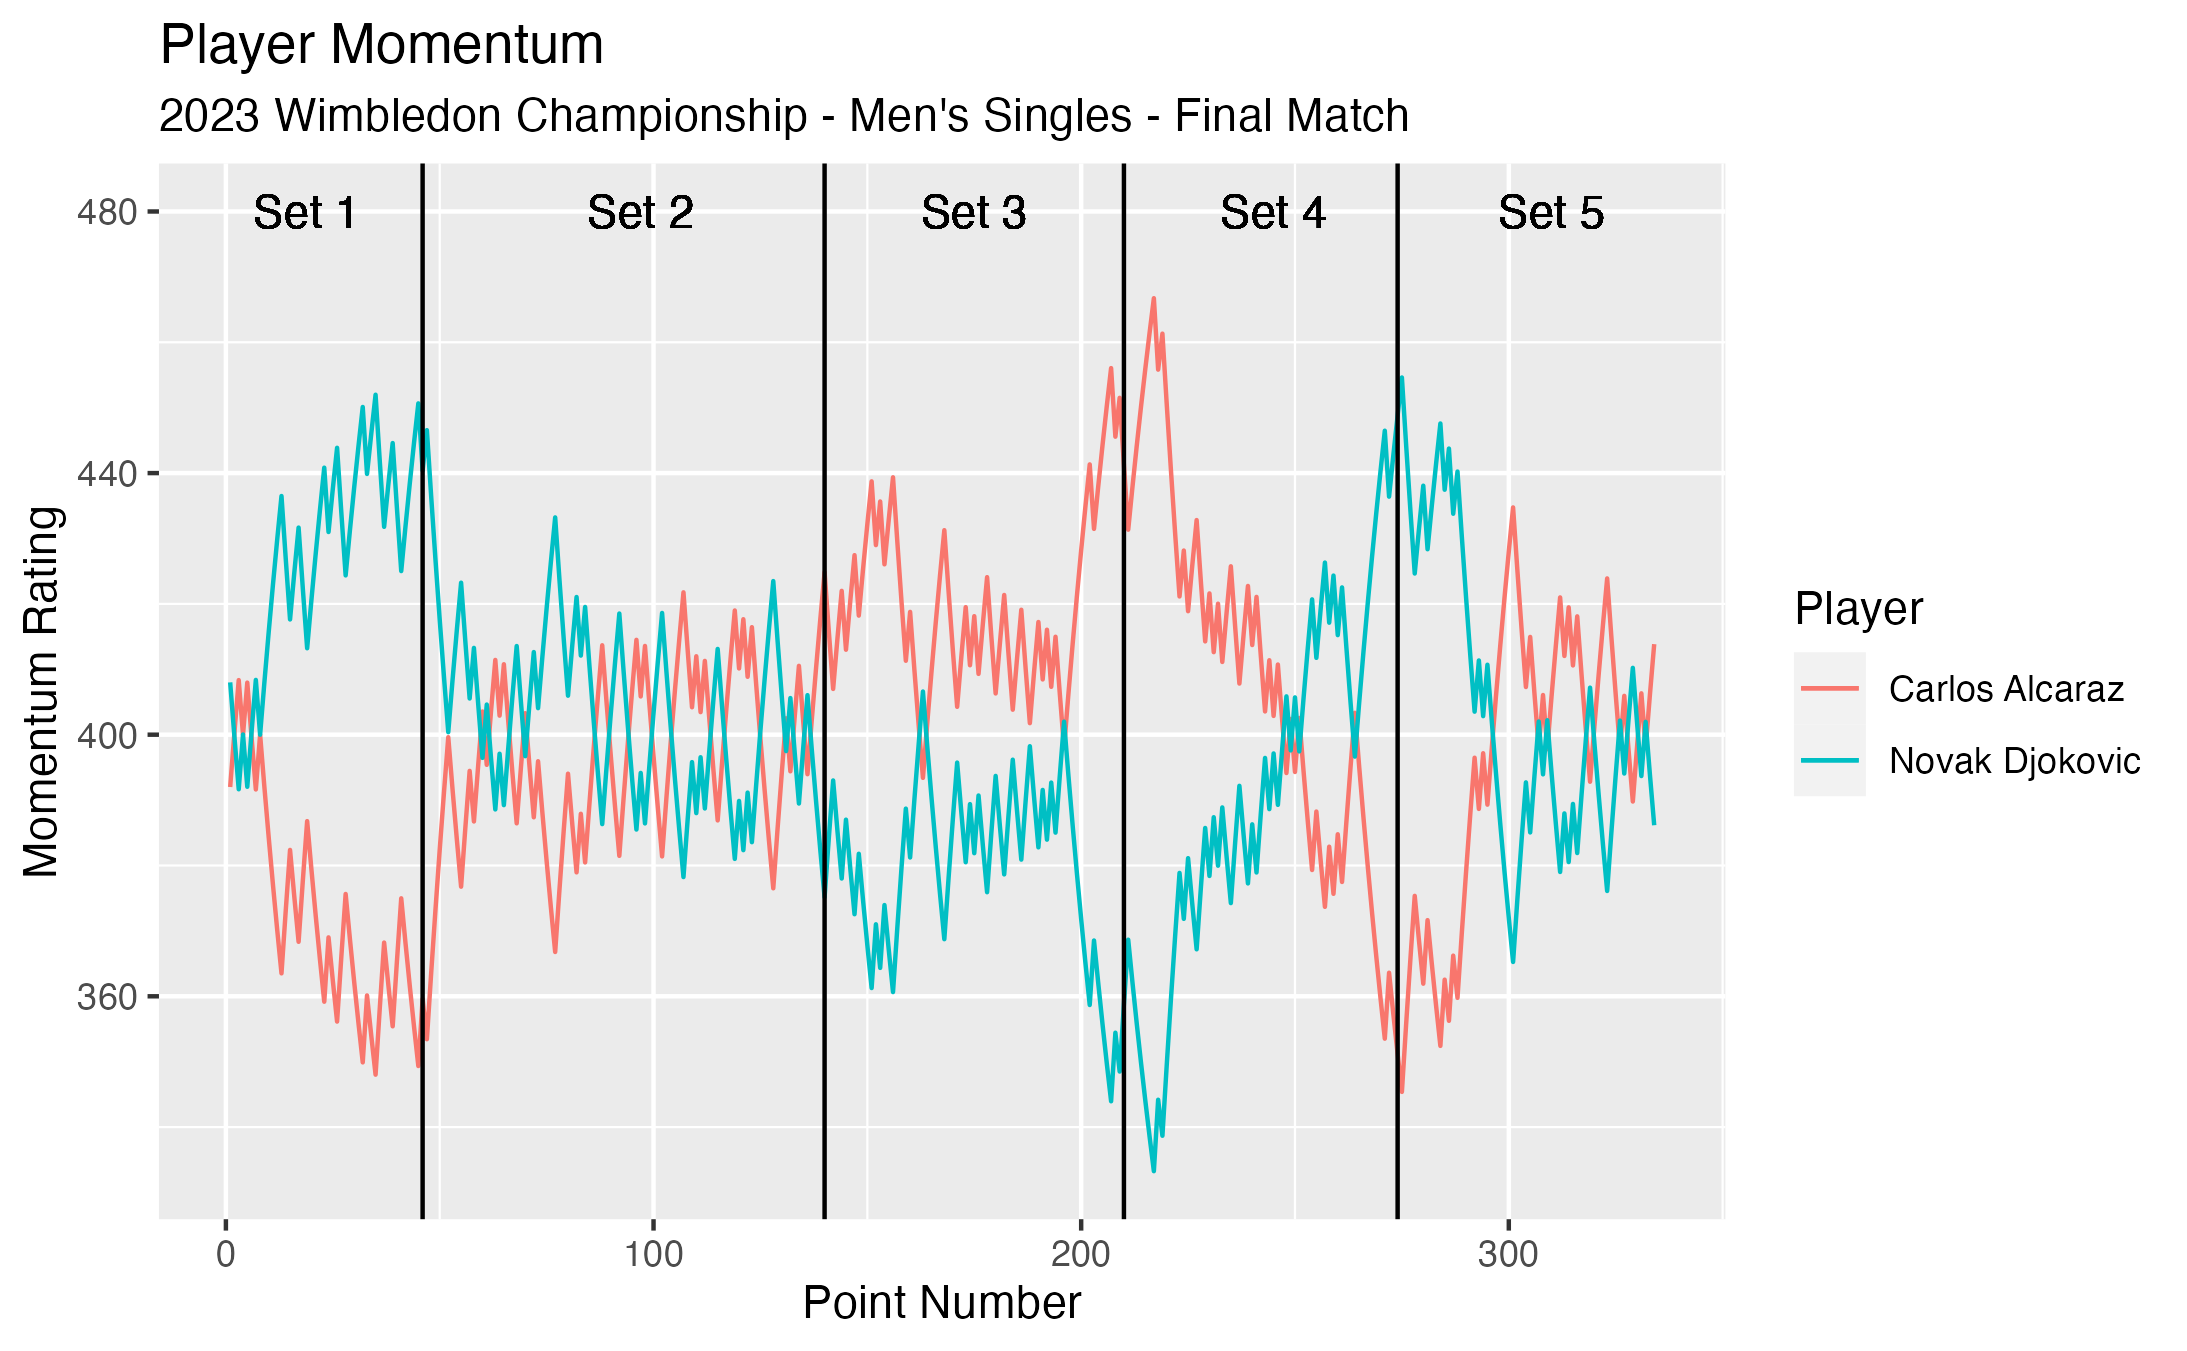
\includegraphics[keepaspectratio, width = \textwidth]{Figures/Final_Match_Player_Momentum.png}
                \caption{Player momentum through the duration of the final match (K=16).}
                \label{fig:Elo_final}
            \end{figure}

            \noindent
            When we apply the formula given in Equation \ref{eq:Elo_Rating_Odds_Formula} to compute the odds of players winning, we can obtain the win probabilities through the course of the match as shown in Figure \ref{fig:Win_Probabilties}.

            \begin{figure}[H]
                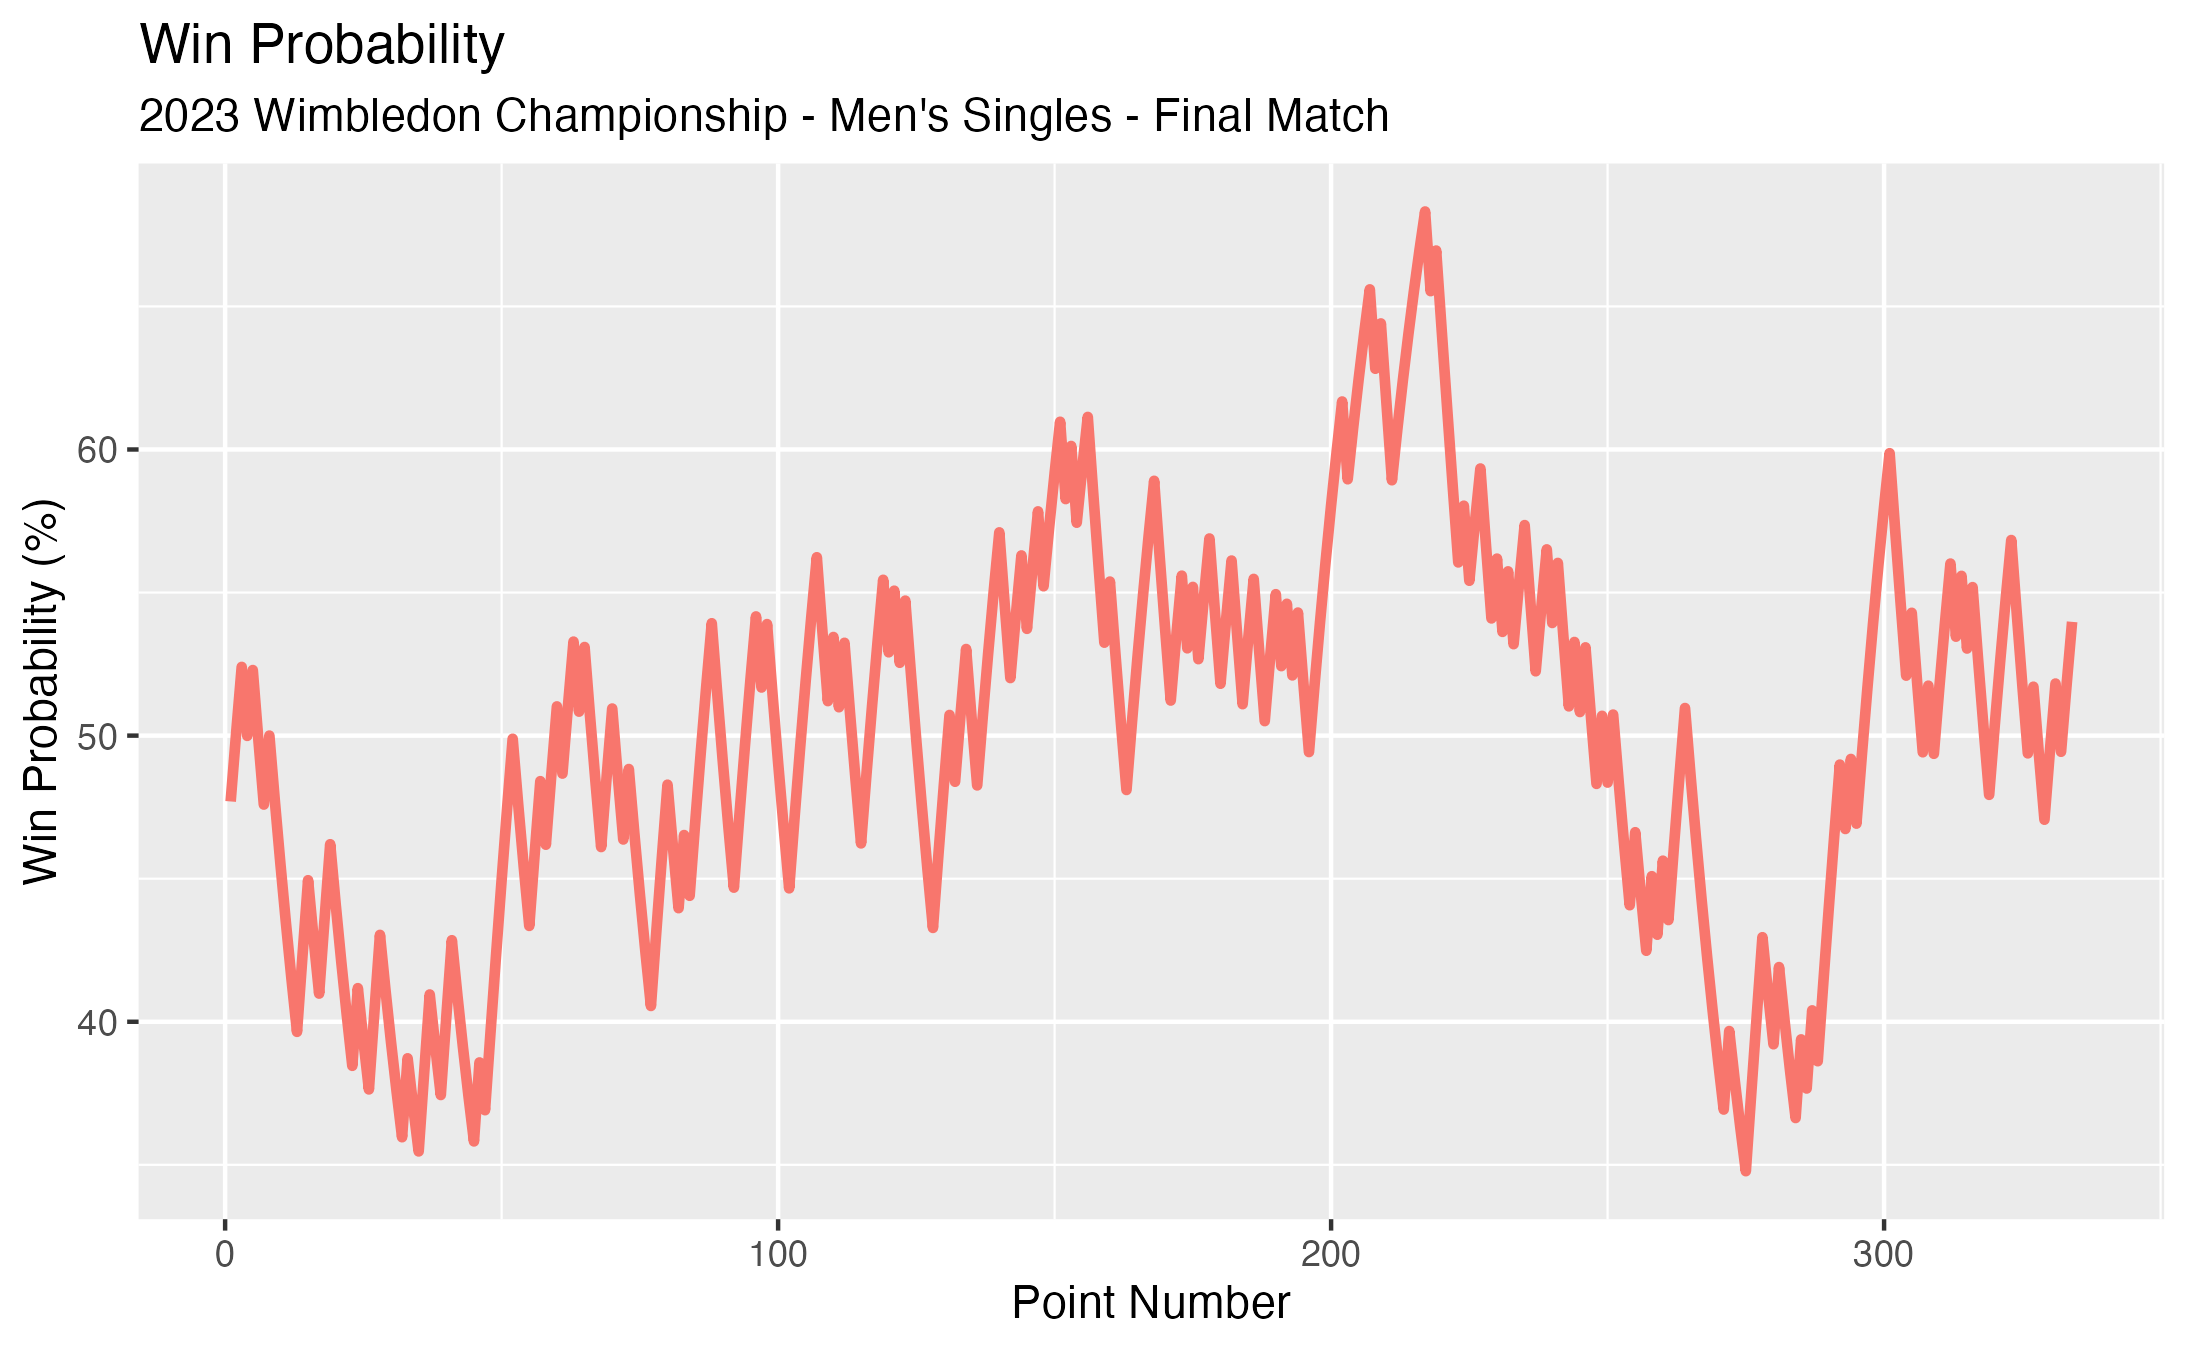
\includegraphics[keepaspectratio, width = \textwidth]{Figures/Carlos_Alcaraz_Final_Match_Win_Probability.png}
                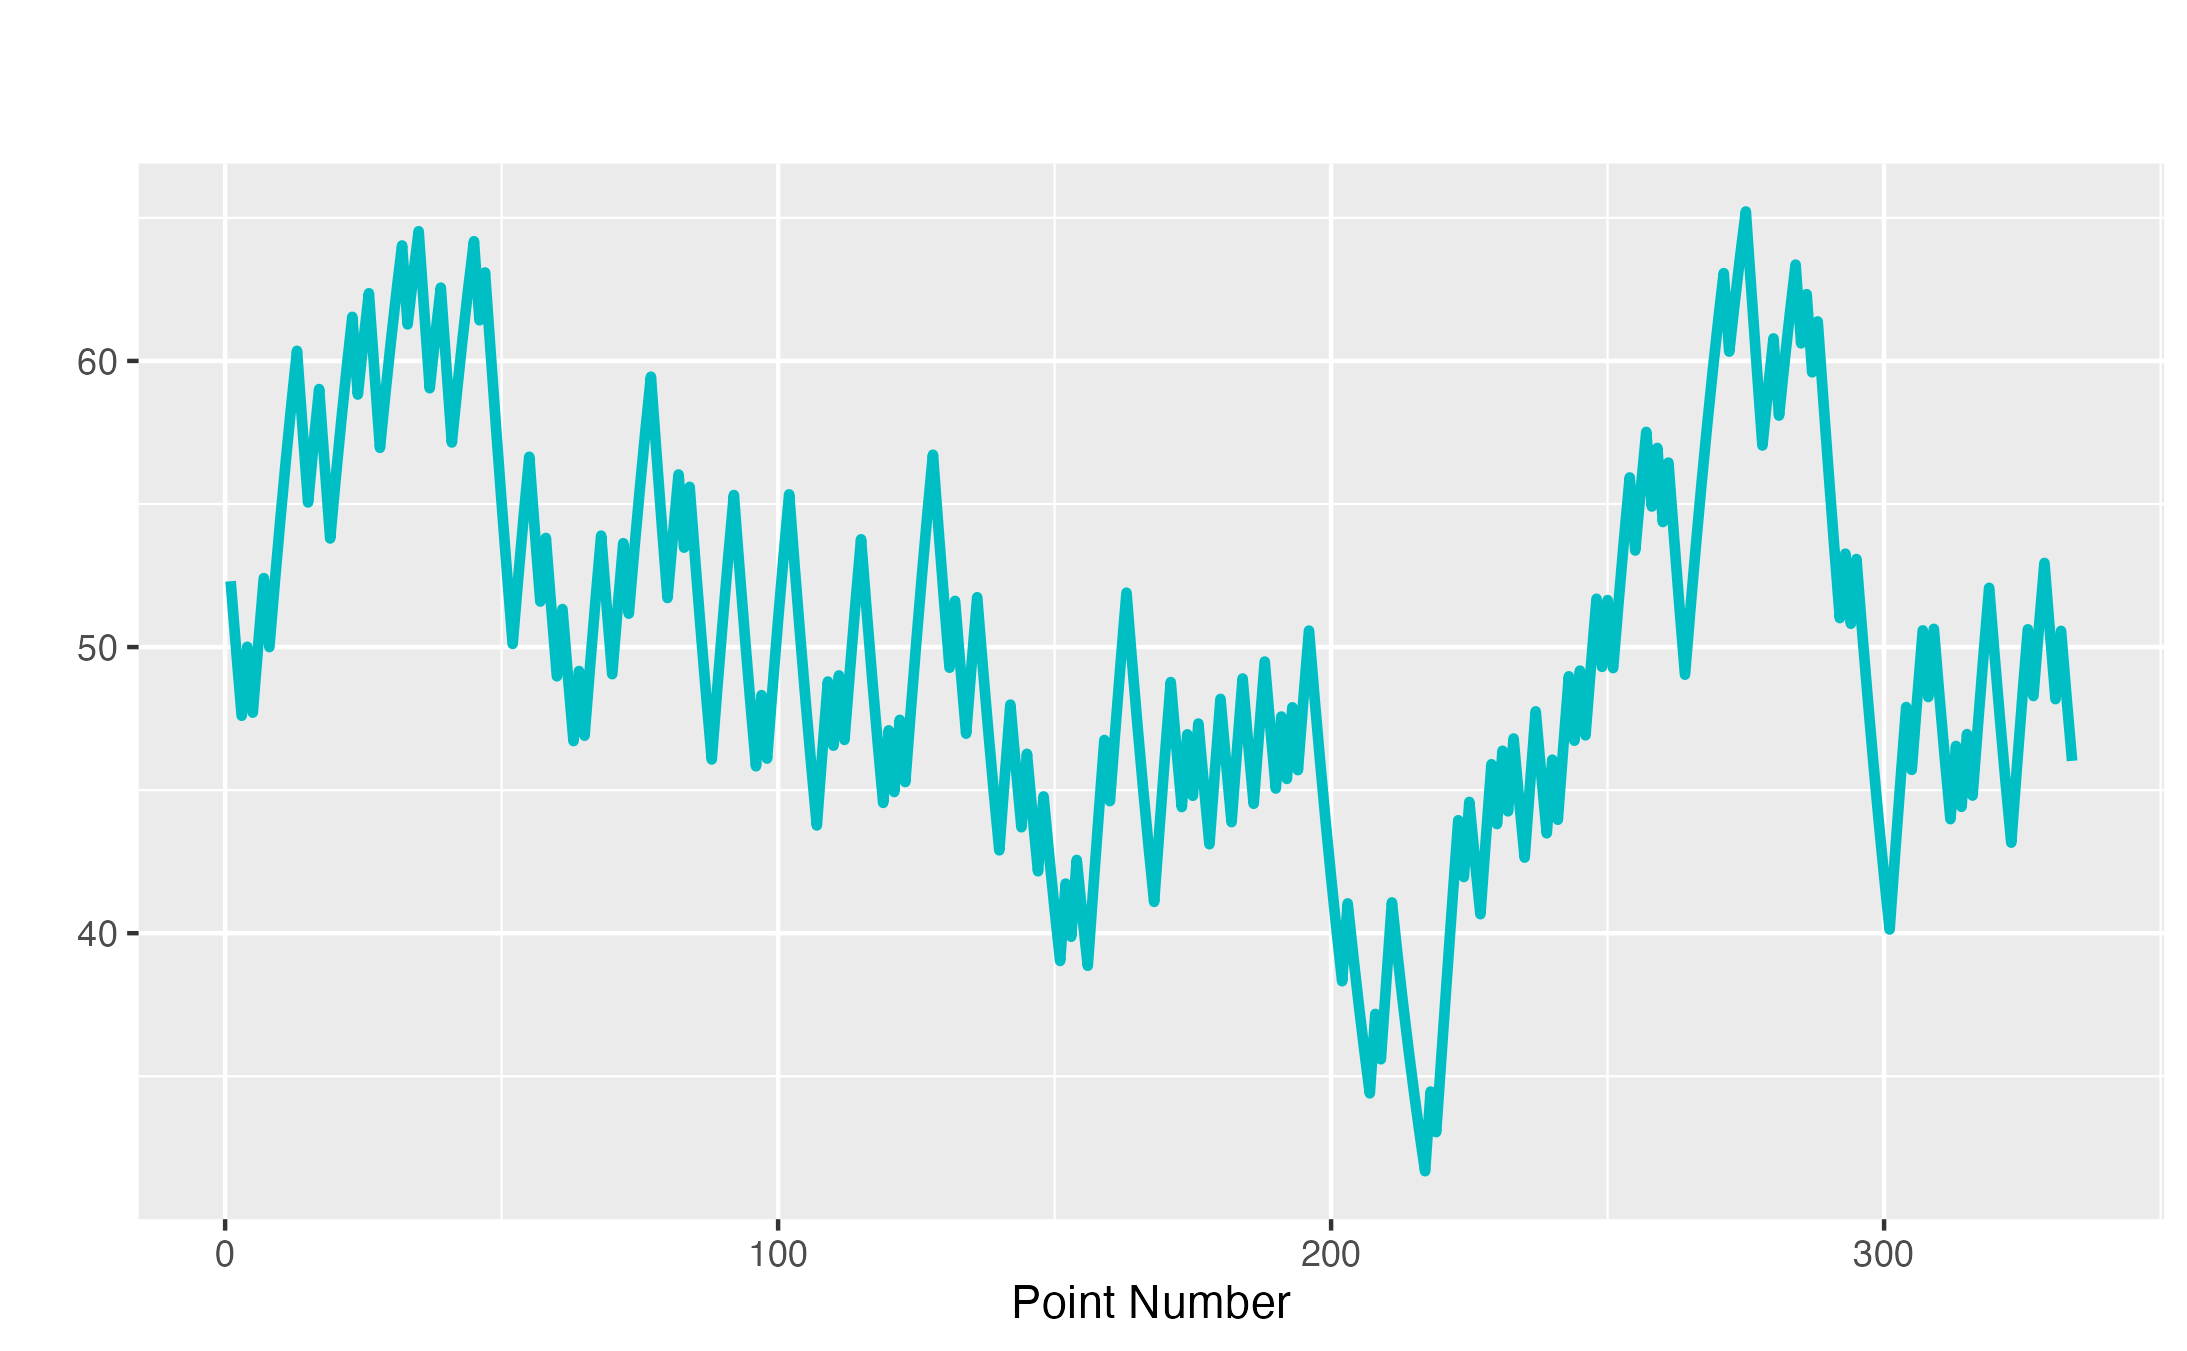
\includegraphics[keepaspectratio, width = \textwidth]{Figures/Novak_Djokovic_Final_Match_Win_Probability.png}
                \caption{Win probabilities of Carlos Alcaraz (Salmon) and Novak Djokovic (Teal) over the duration of the final match.}
                \label{fig:Win_Probabilties}
            \end{figure}

            \noindent
            Notice the movement of the rating of each player as opposing the movement of the rating for the other player (i.e. as one player's momentum increases, the other's decreases and vice versa).

        
        % Momentum Detection
        \subsection{Momentum Detection}\label{sec:Momentum_Detection}

            The Elo rating is computed on a point-to-point basis for both players as they score or lose points. We assume that a single loss or gain of points in the short-term is not representative of the overall trend in momentum of a player. We discuss this assumption in Section \ref{sec:Model_Assumptions}. 
            
            Consider a sequence where players take turns trading points. If we use Elo loss by itself as a measure of momentum, we would incorrectly conclude that a momentum shift occurs at every point. To avoid this situation, we must look at sequences of adjacent points and measure the overall movement trend. To this end, we use a local regression algorithm. 

            \subsubsection{Local Regression}
            Locally weighted scatterplot smoothing (LOWESS) is a non-parametric regression method where a line is fitted to the nearest neighbors of a particular point. By fitting lines to close neighborhoods of the data, we can focus on short-term trends while not overfitting to the back-and-forth trend of points in tennis. In practice, this essentially ``smoothens out'' the Elo/momentum ratings and allows to quantify how well a player is performing during a short sequence of points.
            
            %% insert smoothed momentum difference of final
            \begin{figure}[H]
                \centering
                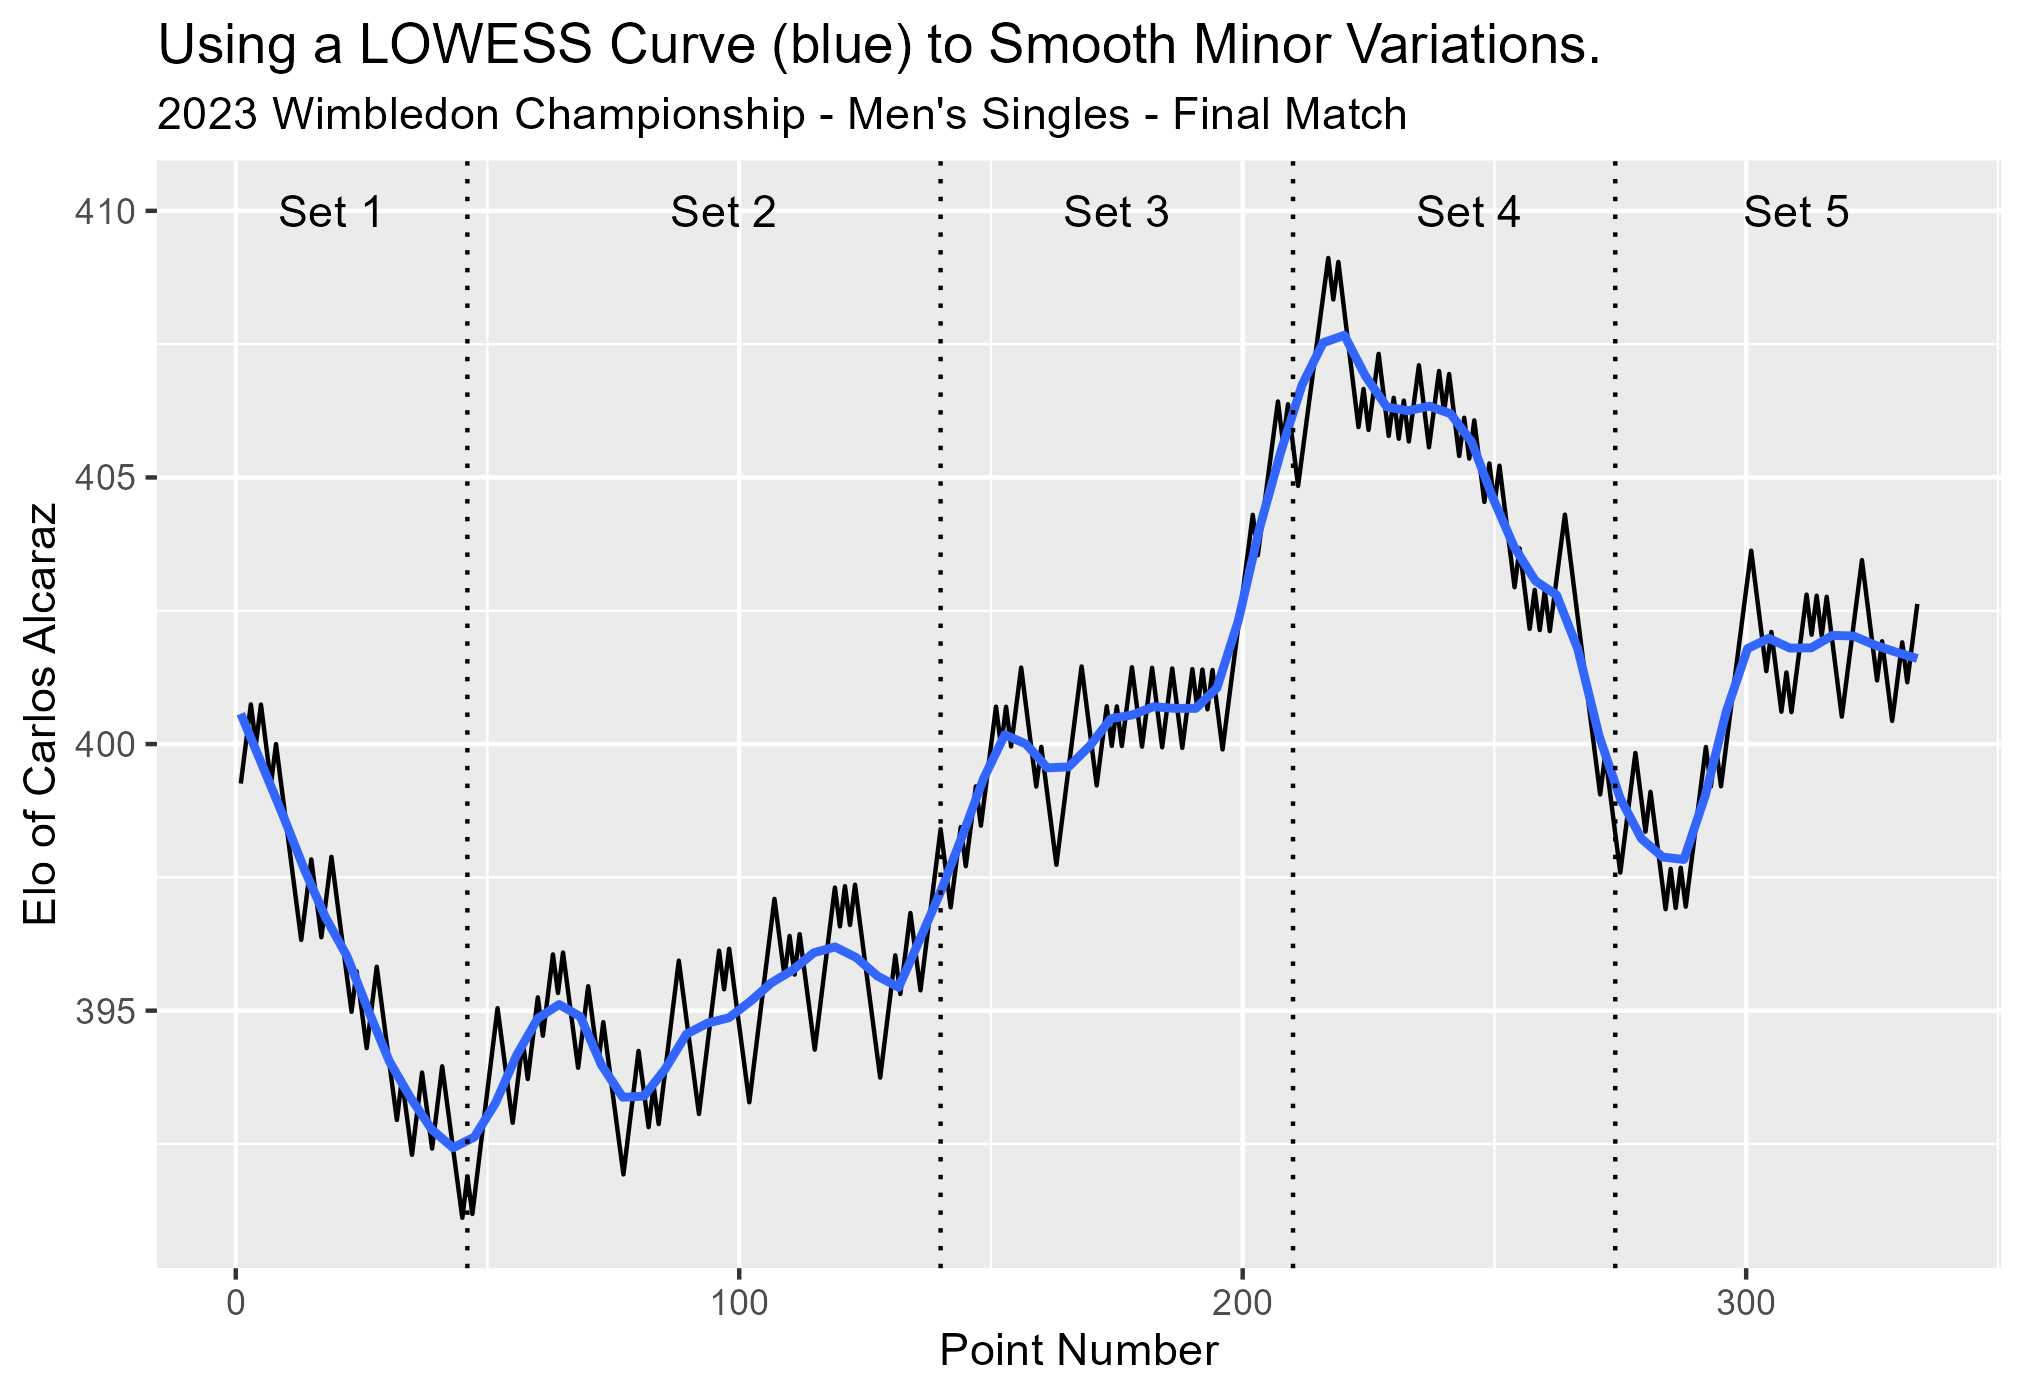
\includegraphics[keepaspectratio, width = \textwidth]{Figures/Final_Smoothed_Diff.png}
                \caption{Smoothed Elo of Carlos Alcaraz during the final match}
                \label{fig:smooth_Elo}
            \end{figure}

            \noindent
            By taking the difference of smoothed Elo between subsequent points in a match, we can measure when a player is performing relatively well compared to the result of the match so far. This is where using Elo score to measure performance has an impact, as, for example, someone winning a series of points while being behind would lead to a larger Elo swing than if that player was already ahead. Compare Figure 3 and Figure 4. The smoothed elo difference is larger when swings in the course of the match occur.
            
            \begin{figure}[H]
                \centering
                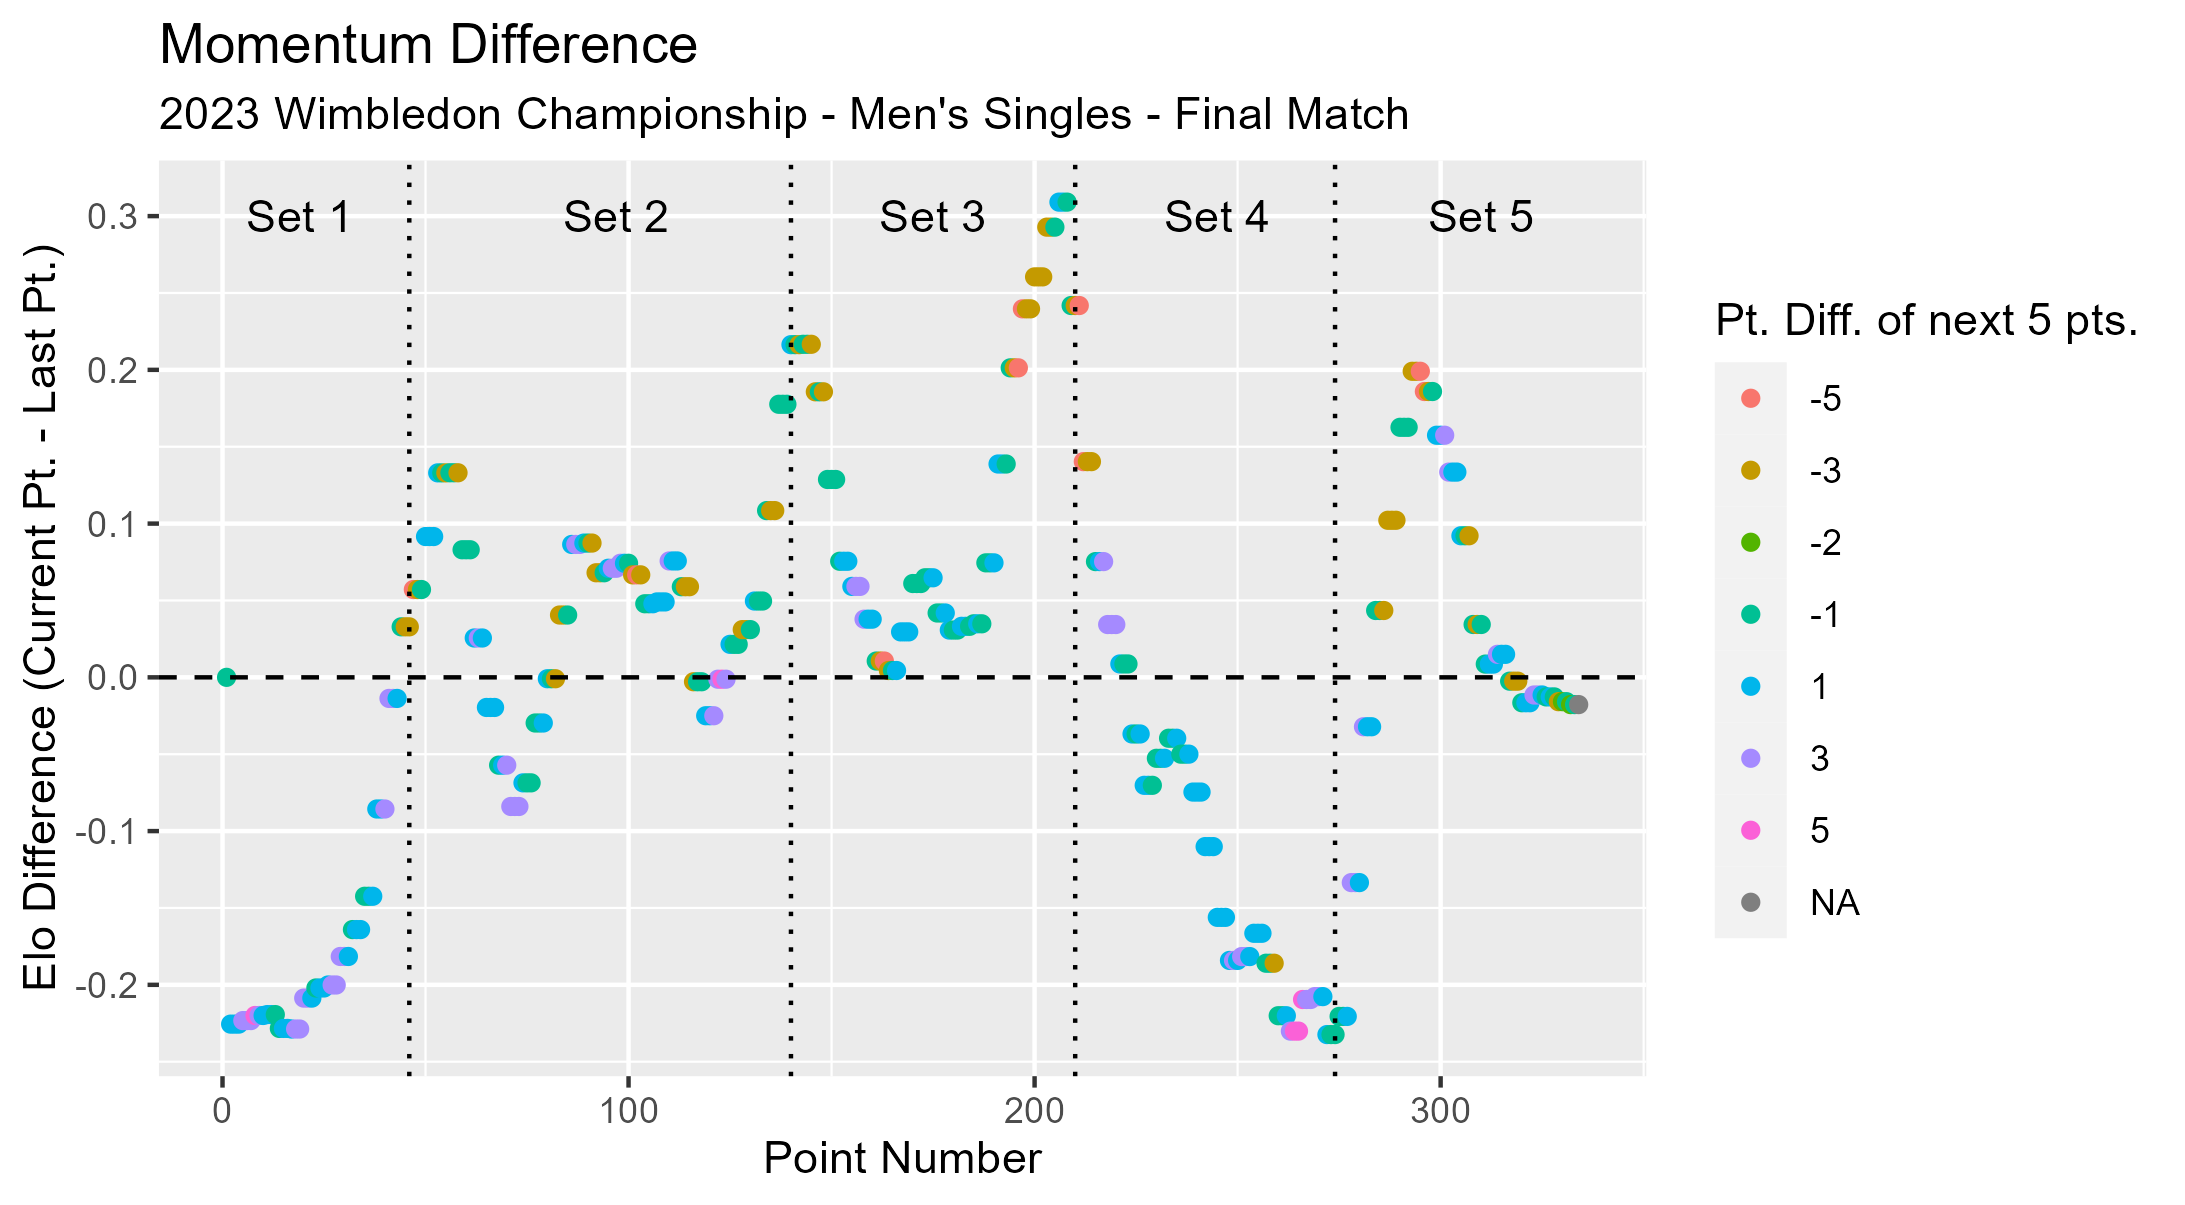
\includegraphics[keepaspectratio, width = \textwidth]{Figures/Final_Match_Momentum_Difference.png}
                \caption{Smoothed Elo Difference during the final match.}
                \label{fig:diff_final}
            \end{figure}

            

            \subsubsection{Training the Appropriate Span}
            When using LOWESS regression the most important hyperparameter is the span, which determines the maximum range of the neighbors used to predict a datapoint. This value is determined as the fraction of all points in a dataset used to calculate the local line. With a large span, points further away are used and vice versa. 
            
            Choosing the span subjectively could introduce a source of error into our analysis, so we chose to optimize this parameter based on how well the resulting momentum metric predicts the point difference in the next 5 rounds. Since the K-factor determines the maximum Elo movement, we decided to optimize the span and K-factor jointly. We also controlled for the serving player while training to remove the source of potential bias. 

            Optimization methods vary wildly in their methodology, so we trained our values according to multiple distinct appropriate methods. We compared a simple random walk, the Conjugate Graduent method, Broden-Fletcher-Goldfarb-Shanno, and Nelder-Mead. All algorithms except for the simple random walk were performed using the \texttt{optim()} function from the base \texttt{stats} package in R. Fortunately, all the algorithms we experimented with converged within three decimal places. We also experimented with different initial starting values for the optimization methods, with similarly negligible results. The final value obtained for span and K-factor were 0.099 and 1.48 respectively. Interestingly, the ideal K-factor was quite far from traditional recommendations by groups that use an Elo system. We suspect this difference comes from the fact that we reset the Elo every match and the elite level of play at Wimbledon.
            
        \subsection{Predicting Momentum}
            %% using stepwise selection to choose the most important variables
        
            %% since we scale them all to 0-1 or an indicator, we can interpret effect size based on the magnitude of the coefficient associated to that variable in a linear model
        Once we have found the optimal hyperparameters for our momentum metric, we can determine which possible events in a point of tennis influence the momentum of a match. We measure this by creating a linear model using smoothed Elo difference as a response variable with the events listed in Section 3 as predictors. However, we don't expect most to be significantly influential, so we have to trim down the space of predictors. We use a step-wise selection algorithm to efficiently remove unimportant features.

        \subsubsection{Step-wise Selection}

        Stepwise selection is a feature selection technique that iteratively decides the best model out of a group of possible predictors by, at each step, starting with a current model and finding the best model obtained by adding or removing one predictor. The algorithm stops when no addition or deletion improves the model. The main point of variety in different stepwise selection algorithms is how to determine whether a model is ``good'' or ``bad''. The most common ways to measure model ``goodness'' are the Akaike Information Criterion (AIC) and the Bayesian Information Criterion (BIC). These metrics vary in how heavily they penalize a model for having more variables, with AIC favoring having more predictors in a model compared to BIC. Since we only want to remove variables that have almost no impact on the model, AIC is more appropriate. For the same reason, we choose to start the stepwise selection with a model containing all variables. 
        
        The final model we obtained through this selection process contains these following predictors: set number, game number, point number, sets won, games won, points won, winning shot type, unforced errors, net points, break point, break point wins, distance run during a point, and serve width.

        \subsubsection{Interpreting the Final Model}
        Unfortunately, the stepwise selection algorithm only tells which predictors have an impact rather than how much impact they have. However, we can measure the influence of variables using their coefficients in the final linear model. This introduces one final roadblock to a meaningful answer: Some variables are on different scales. For example, most predictors are indicators, which means that they record whether something happens or not as a one or a zero. However, a variable like distance run by a player is measured in meters, so a unit increase means something entirely different than a predictor like whether a break point is won or not. Luckily, distance run was the only unscaled variable which significantly affects the momentum rating. We transformed this variable to a range of 0 to 1 by dividing the distance run in each point by the maximum distance run over the entire tournament. Finally, we obtain a measure of which possible events in a tennis match influence momentum the most.

        \begin{table}[]
            \centering
            \begin{tabular}{c|c}
                Predictor & Effect on Smoothed Elo Difference \\ \hline
                Winning a Break Point &  0.137\\
                Distance Run & 0.115 \\
                Participating in a Break Point & 0.042 \\
                Having an Unforced Error & .037 \\
                Winning with a Backhand Shot & .034
            \end{tabular}
            \caption{The five most influential predictors of momentum.}
            \label{tab:my_label}
        \end{table}

        The most influential factors in predicting momentum swings are winning break points and distance run. This provides a counterpoint to the argument that momentum is completely random, as we would see uniform effect sizes across all variables.
    % Model Analysis
    \section{Model Analysis}
    
        % Model Limitations
        \subsection{Model Limitations}

            Elo ratings have certain limitations that should be considered. Firstly, ratings are based on an interval scale, thus they are relative and lack an absolute meaning \cite{Elo1986}. It is meaningless to talk about the ratio of ratings between two players (i.e. ``The rating of Player A is $x$ times higher than the rating of Player B"). There is no standardized defnition of a specific Elo rating as stratification of players by rating varies across games, organizations and may change over time. \\

            \noindent
            With regards to modeling momentum in tennis matches, without enough points to a player's Elo rating, the ratings that have been calculated for a particular set of matches do not generalize when rated players play against a different set of individuals. Furthermore, if two players haven't been previously ranked and are defined to have the same initial Elo rating, the model interprets them to have the same odds of winning, which may or may not be true depending on other factors that are not accounted for in the model.
    
        % Model Assumptions
        \subsection{Model Assumptions} \label{sec:Model_Assumptions}

            As mentioned in Section \ref{sec:Momentum_Detection}, the momentum rating is calculated on a point-to-point basis, resulting in short-term fluctuations in the rating. Our model assumes that these fluctuations are not indicators of medium- to long-term gain or loss in momentum. Realistically, if a player wins successive points, loses one or two points, and then wins enough points to win the set, the lost points shouldn't imply that they lost momentum. We observe this in other sports as well. For example, in American football, if a team makes successive first downs\footnote{Advancements of 10 yards towards the opposing team's endzone}, fails to make first attempt first-down (i.e. they require two or three attempts to make the next set of downs), and then makes another first down, they are not said to have lost momentum. 

        % Model Strengths
        \subsection{Model Strengths}

        Due to the smoothing by the LOWESS regression, the model is robust to the influence of any one point and instead accurately reflects larger trends, making it an ideal representation for the flow of a match. 

        This model also has the ability to model the momentum over varying scopes, ranging from over the duration of a single match to an entire tournament or even a set of professionals' careers. In the case that a single match is modeled, the rating of the two professional can be considered the same at the start, so that only the ``swings'' throughout the match are captured in the momentum without a starting bias. In the case of a large tournament, players within a match might start with different ratings, reflecting their previous successes, so that the momentum corresponds to the player who is projected to win at the start. Furthermore, the K-factor can also vary with the progression of a tournament, so that the amount that the momentum changes by can be made larger or smaller at critical points in the game. This allows the model to reflect the increase in the tension perceived at later games in a tournament. To model a group of players over multiple years, it is only necessary for the starting ratings of players to be consistent relative to one another. This can be done by either starting off with a single rating for everyone, or, if enough historical data is available, by calculating relative ratings using the fact that differences in Elo ratings correspond to the odds of the player with a higher rating winning, as outlined in equation \ref{eq:Elo_Expected_Scores} \cite{Elo1986}.

        Because this method can model the momentum of any two players by starting with identical ratings for both, it the ability to generalize across many different factors, including gender, court surfaces, or potentially even other sports, becoming more accurate with increased access to historical data. 
        
        


% on the last bullet point, where they talk about a 25 page report, they say: " include a one- to two-page memo summarizing your results with advice for coaches on the role of “momentum”, and how to prepare players to respond to events that impact the flow of play during a tennis match"

        
    % Validation and Verification
    \section{Validation}

        % Sensitivity Analysis
        \subsection{Sensitivity analysis} \label{sec:Sensitivity_Analysis}

            One primary source of debate when utilizing Elo ratings is the optimal selection of the K-factor. In his original article, Elo discussed the implications of different values of K, noting how novice players tend to learn faster and using a higher value of K to reflect this. As mentioned in section 4.2.2, the optimal K value of 1.48 was significantly smaller than those traditionally used to rank chess matches, which, along with the relatively small span value of 0.099, agrees with the intuition that at the elite level, the advantage changes are subtle. A similar effort to ours involving basketball win prediction utilized Elo ratings and found that even when the K-Factor was optimized over, the value of the K-Factor showed no difference in prediction power \cite{Dobson2019}. This reinforces our selection of the Elo rating method as a simple and robust method.

    % Memo to Coaches and Players
    \section{Memo to Coaches and Players}
    
        Our research into the presence and effect of momentum has lead us to two main conclusions. First, momentum does not appear to be random. To show this, we used a smoothed Elo system to find points over the course of a match where the flow changes. This is an improvement over using simple point differential as it weights situations where a player wins a point while losing more heavily than a player extending their lead. Once we quantified momentum, we used statistical methods to determine what events during a point most influence momentum. We find that winning break points and running large distances during a point increase a players momentum. This leads us to our recommendations: \textbf{Incorporate heavier cardiovascular exercise into practice regimes and use mindfulness exercises after losing games in a set to ground oneself.}
        
        The benefit of cardiovascular exercises is straightforward. Being less tired after running large distances will allow players to capitalize on their momentum advantage more effectively. We find the second recommendation to be more interesting. We attempt to mitigate the momentum advantage an opponent receives after winning a break point. By realizing that momentum changes not with each point but over a series of points, players can help calm themselves in the occasion that they lose one or even multiple points, knowing that there is more to their momentum than just the immediate few scores. Conversely, after winning a break point yourself, playing with more confidence will lead to more negative mental impact for the opponent. While we don't recommend behaving in an unsportsmanlike manner, strong celebrations after winning break points may also increase this advantage. Players can also feel better about gaining a single point while they feel like they have less momentum, since their disadvantage is factored into the Elo ranking. Similarly, coaches can keep this phenomena in mind and maintain an encouraging attitude that can help create a positive environment for the player, boosting their confidence and inevitably positively affecting their outlook on their own performance. While the Elo model relies on observable and measurable aspects of the game, it is understood that the psychological state of a player is one of the factors that impacts their performance, and it is also important for players to maintain a calm and positive state of mind in order to put maximum mental effort towards the match. 
    
    % References
    \printbibliography

\end{document}
